\documentclass{article}

\usepackage{amsmath}
\usepackage{amssymb}
\usepackage{graphicx}
\topmargin=-1in
\evensidemargin=0in
\oddsidemargin=0in
\textwidth=6.5in
\textheight=9.0in
\headsep=0.25in

\begin{document}
\title{\textbf {Hoja de Trabajo No. 1}}
\author{Sebastian Gomez}
\maketitle

\textbf {EJERCICIO NO.2}

\begin{center}
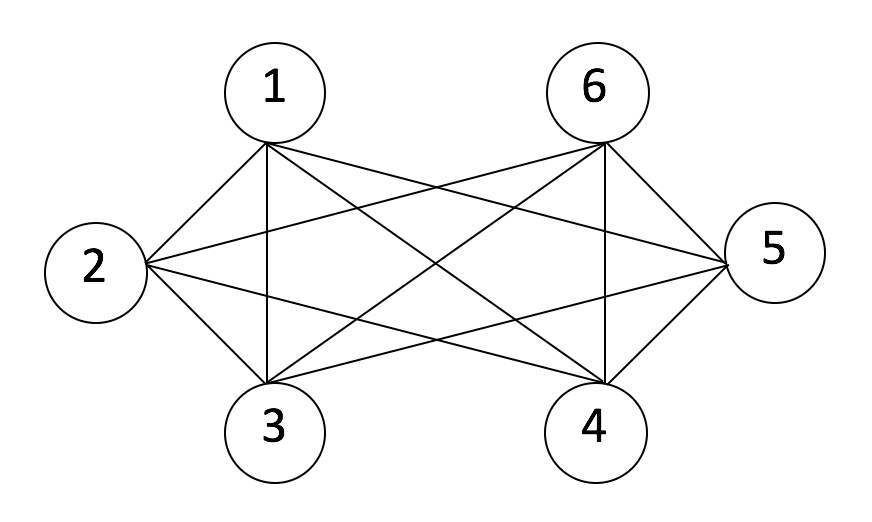
\includegraphics{grafo dados.png}
\end{center}
\begin{enumerate}
[$<1,2>$ $<1,3>$ $<1,4>$ <$1,5>$ $<2,3>$ $<2,4>$ $<2,6>$ $<3,5>$ $<3,6>$ $<4,5>$$<4,6>$ $<5,6>$]
\end{enumerate}


\textbf {EJERCICIO NO.3}
\begin{enumerate}
\item La estructura de datos que representa un lanzamiento de dados es un grafo bipartito.
\item El algoritmo que yo creo que se acopla más a este grafo es el algoritmo de Kruskal.
\item El algoritmo funciona porque tiene vias para ir a cuatro de 5 vertices por lo que puede ir para donde sea. 
\end{enumerate}





\end{document}
